\documentclass[]{i3thesis}
% options:
% [germanthesis] - Thesis is written in German
% [plainunnumbered] - Don't print numbers on plain pages
% [earlydraft] - Settings for quick draft printouts
% [watermark] - Print current time/date at bottom of each page
% [phdthesis] - switch to PhD thesis style
% [twoside] - double sided

\usepackage{multirow}
\usepackage{floatflt}
%\usepackage[babel=true]{csquotes}
%\usepackage[backend=biber,style=ieee]{biblatex}

\author{Dustin Heither}
\title{Flexible and Efficient QoS Provisioning in AXI4-Based Network-on-Chip Architecture - A brief comprehension}
\thesistype{Paper in the subject Neuartige Rechnerarchitekturen}
\thesiscite{Seminar Paper}
\birthday{10. May 1992}
\birthplace{Oberhausen}
\thesisstart{1. April 2025}
\advisors{M.Sc. Philipp Holzinger}

\addbibresource{thesis.bib}
\graphicspath{{images/},{pictures/}}

%%%---------ADD EVALUATION-----------------------------------
%\newcommand*{\WITHEVALUATION}{}%
%%%
\begin{document}
%%%----------------------------------------------------------

\pagenumbering{roman}

\maketitle

% Uncomment \input macros as required
%\input{abstract}
\acresetall

\cleardoublepage
\tableofcontents

\cleardoublepage
\pagenumbering{arabic}

\chapter{Introduction}

As part of the seminar “Neuartige Rechnerarchitekturen”, the paper “Flexible and Efficient QoS Provisioning in AXI4-Based Network-on-Chip Architecture” by Wang and Lu (2022) is analyzed in detail.\cite{wang_flexible_2022} The goal of this analysis is to engage deeply with the presented architecture, identify key concepts and findings, and prepare a seminar presentation that clearly conveys these to fellow students.
The seminar is part of the Bachelor's program in Computer Science at Friedrich-Alexander-Universität Erlangen-Nürnberg and was attended during the summer semester of 2025.

The title of the paper already points to three essential core aspects: \ac{QoS}, \ac{AXI4}, and \ac{NoC}. These terms will be explained in more detail, placed in their technical context, and examined in relation to each other. The objective is to provide a comprehensive overview and analysis of the architecture developed by Wang and Lu.

With the increasing number of processor cores and functional units in modern \ac{SoC} designs, the demands on efficient and reliable communication between these components also grow. For this reason, NoC architectures are becoming increasingly important. At the same time, many applications require low latencies and guaranteed bandwidth, making flexible QoS support essential. The AXI4 standard has become a widely adopted protocol in the industry, highlighting the relevance and timeliness of the approach presented by Wang and Lu.\cite{jake_ke_demystifying_2025}\cite{gomez-rodriguez_survey_2021}\cite{talwar_traffic_2013}

To provide technical context, the key concepts (\acs{NoC}, \acs{QoS}, and ˜\acs{AXI4}) are first compared with the current state of the art and relevant research literature. This is followed by a detailed description of the architecture introduced by Wang and Lu, including discussion of the role of the subnetworks (\ac{VC} and \ac{TDM}) and the \ac{NI}. Building on this, the experimental results are presented and critically evaluated.


\chapter{Background and State of the Art}

\section{Network-On-Chip}

\sh{Evolution of Buses}
A network-on-chip is a communication system used in modern \ac{SoC} architectures to efficiently connect various components (e.g., processors, memory, and specialized units). Instead of using classic buses or point-to-point connections, \ac{NoC} relies on a network-like communication principle inspired by computer networks or high-performance computers.~\cite{serpanos_architecture_2011}

The Fig.~\ref{fig:Evolution_of_Interconnection} shows the development of bus technologies over the past few years.
\begin{figure}[htbp]
    \centering
    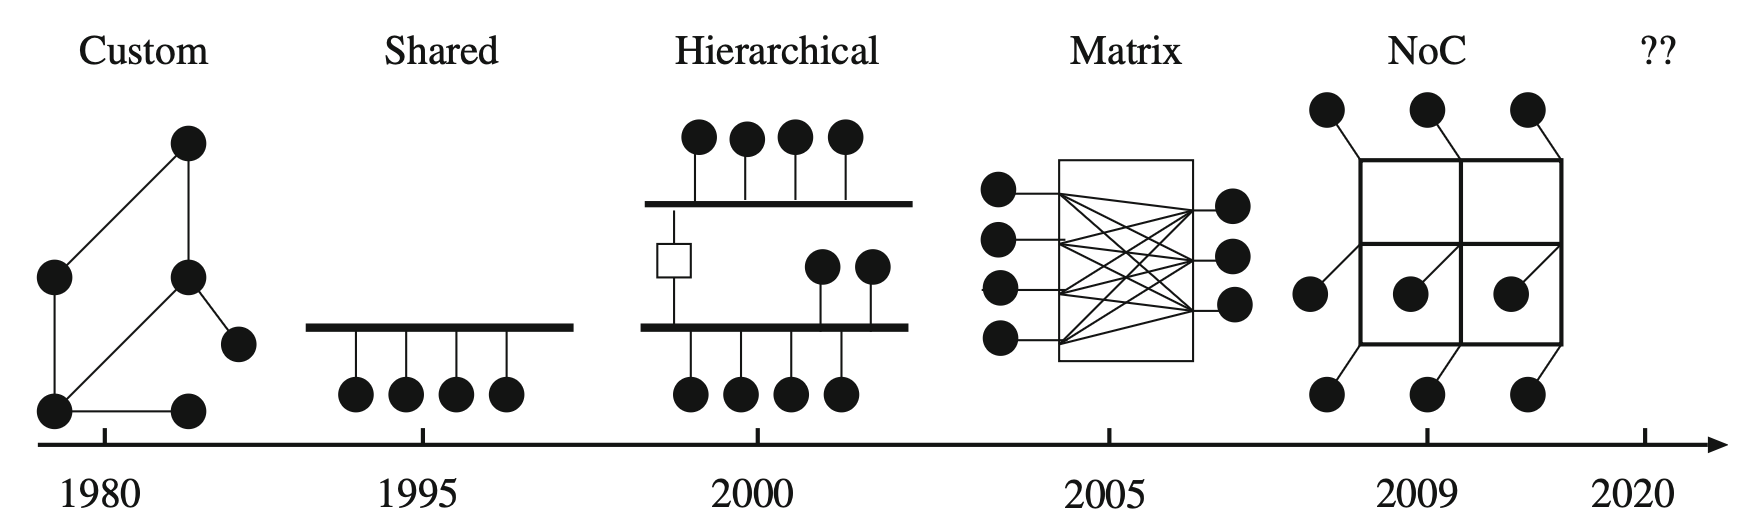
\includegraphics[width=0.95\textwidth]{img/Evolution of On-Chip communication interconnect.png}
    \caption{Evolution of Interconnections}\cite{abderazek_multicore_2013}\label{fig:Evolution_of_Interconnection}
\end{figure}

Before 1980, custom solutions were typically used for on-chip communication. Starting around 1995, so-called shared-bus architectures such as ARM’s AMBA bus \cite{arm_amba_nodate} and IBM’s CoreConnect\cite{international_business_machines_corporation_coreconnect_1999} were introduced. These approaches enabled a more modular design with standardized interfaces and supported the reuse of IP components (IP reuse).


However, as bandwidth demands increased, shared-bus systems became a bottleneck. To address this issue, hierarchical bus architectures were introduced. These utilize multiple buses or bus segments to reduce the load on the main bus. Local communication between modules on the same bus segment is possible without burdening the entire bus. Nevertheless, such architectures are only limitedly scalable, inflexible, and lead to increased design complexity. The more cores are connected, the harder it becomes to meet timing constraints (time closure\footnote{Time Closure: Successfully ensuring all timing constraints are satisfied in the design so that the chip can operate reliably at its target clock frequency.}) and ensure \ac{QoS}.


Another alternative was the bus matrix — a full crossbar system that allows parallel connections between components. However, as system size grows, the complexity of wiring also increases and can eventually improve the effort required for the logic itself. Moreover, such systems do not clearly separate transport, transaction, and physical layers. Therefore, when a system upgrade is needed, it often affects the entire interface design and all connected blocks.


Against this background, some researchers in the early 2000s proposed implementing communication between different processing units on a chip via a predefined platform—an integrated switching network known as Network-on-Chip. NoCs fulfill key requirements of modern \ac{SoC}s: Reusability, scalable bandwidth, and energy efficiency. NoCs have replaced wired connections and instead utilize intelligent network infrastructures. They draw on models, techniques, and tools from network communication, thereby replacing fixed wiring with packet-based communication.\cite{unnikrishnan_network_2021}


\sh{NoC Components}
A \ac{NoC} consists of the following three essential components:\cite{yu_flexible_2010}\cite{unnikrishnan_network_2021}


\begin{enumerate}
    \item \textbf{Links}, which physically connect the nodes and enable communication between them. A link connects exactly two routers (see item 2). A link can contain one or more logical channels; a channel in turn consists of a set of wires (cables). The implementation of a link also includes the definition of the synchronization protocol between the source and the destination node.
    \item \textbf{Routers}, which are responsible for implementing the communication protocol. A router has multiple input and output ports as well as a switching matrix that establishes the connection between these ports. Additionally, each router has a local port connected to the respective IP core. A logic block inside the router controls the flow control (see below for further description) policies and defines the overall strategy for data forwarding.
    \item \textbf{\ac{NA}} or \textbf{\ac{NI}} serve as the logical interface between the IP cores and the network. They are necessary because the internal communication mechanisms of an IP core (e.g. bus protocols like AXI) are typically not directly compatible with the packet-based mechanisms of a \ac{NoC}.
\end{enumerate}


\sh{Topology}
\ac{NoC} can be characterized by the structure of their router connections. This structure is also referred to as the \textit{topology} and is typically represented as a graph $G(N, C)$, where $N$ denotes the set of routers (nodes) and $C$ the set of channels (edges). A fundamental distinction is made between \textit{direct} and \textit{indirect topology}.


In the case of \textit{direct topology}, each router is assigned exactly one processor. This pair is considered a node in the network. Each node is connected to a fixed number of neighbors, and messages are transported over one or more intermediate nodes (routers). Commonly used structures include n-dimensional grids, mesh topologies, or torus topologies (also called k-ary n-cubes).


In \textit{indirect topology}, not all routers are directly connected to a processing unit, as is the case in the direct model. Some routers serve solely to route messages through the network, while others are responsible for control and management functions. These so-called logic routers act as sources or targets of messages.\cite{unnikrishnan_network_2021}


\sh{Routing}
In \ac{NoC} architectures, routing is a central component because it determines how data packets are transmitted between individual nodes. Fundamentally, routing algorithms can be divided into two main categories: deterministic and adaptive routing. 


In \textit{deterministic routing}, the path a packet takes from the source to the destination is predefined and remains unchanged regardless of the current network load or other conditions. Well-known deterministic methods include XY-routing and \ac{DOR}.\cite{ma_summary_2024} 

In contrast, \textit{adaptive routing} allows dynamic path adjustments based on the current state of the network. This enables, for example, the avoidance of congestion or faulty connections. Adaptive algorithms include \ac{DyAD}\cite{hu_dyad_2004} as well as Odd-Even routing.

Complementing these are \textit{congestion-aware routing algorithms} that specifically consider the current network load to achieve an even distribution of data traffic.\cite{fang_parrouting_2020} A special subcategory are so-called \textit{ant colony-based algorithms}, which use concepts from swarm intelligence. Here, paths are learned and continuously optimized using virtual pheromone trails, enabling flexible and adaptive route finding.\cite{luneque_routing_2013}


\sh{Flow Control}
Another essential aspect in \ac{NoC} systems is the so-called flow control, which defines how available resources such as bandwidth or buffer memory are assigned to individual data packets. The goal is to ensure efficient resource usage and thereby optimize the overall network throughput. Fundamentally, one distinguishes between bufferless and buffered flow control. 

In \textit{bufferless flow control}, there are no or only very limited intermediate storage; data packets that cannot be forwarded immediately are either discarded or rerouted via alternative paths. A typical example is circuit switching, where a fixed path through the network is reserved prior to data transmission. In contrast, buffered flow control temporarily stores data packets when the desired output channel is occupied or forwarding is otherwise delayed. This method increases the flexibility of data transmission and reduces the likelihood of packet loss or rerouting, but entails higher hardware complexity and energy consumption due to the additional buffer resources that must be provided and managed.

Within \textit{buffered flow control}, two central approaches can be distinguished: In packet-buffer flow control, the entire packet is stored in a buffer until it can be forwarded completely. This method is simple to implement but can be inefficient, especially for large packets and limited buffer memory. A finer control is provided by flit-buffer flow control, where packets are divided into smaller units called flits (flow control digits) and buffered individually. This allows more efficient use of available memory and better coordination of data flow, potentially leading to higher network performance.

Additionally, different buffering strategies exist within these approaches, including \textit{input buffering}, \textit{output buffering}, and \textit{virtual channel buffering}. Input buffering stores incoming data streams at each input channel, while output buffering places buffers at the router’s output channels. Virtual channel buffering allows multiple logical channels to share one physical channel, thereby reducing blocking and improving the utilization of available bandwidth. However, this technique requires more complex control logic and increases hardware overhead.\cite{dally_principles_2004}

\begin{figure}[htbp]
    \centering
    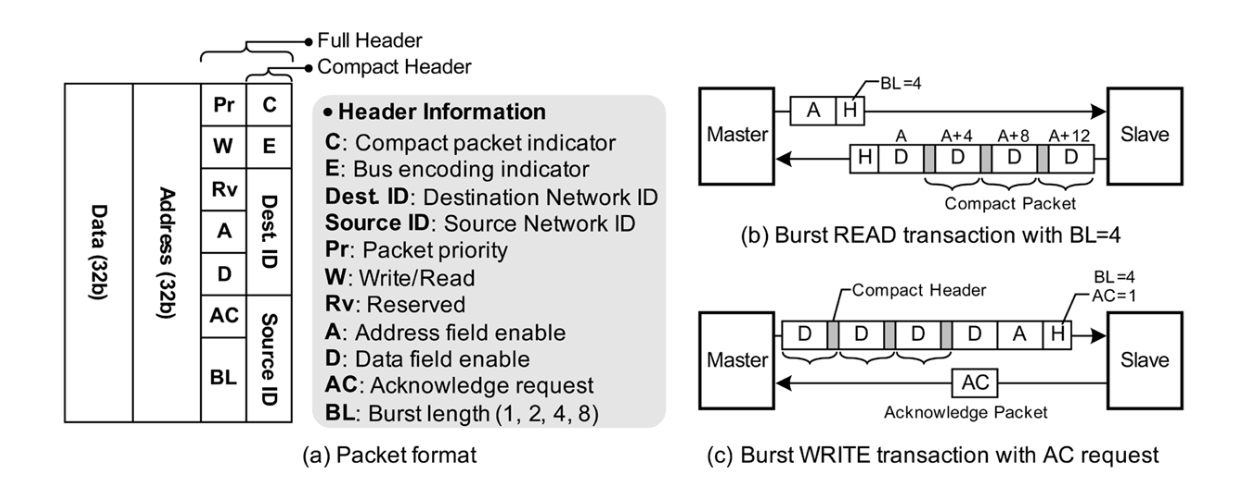
\includegraphics[width=0.95\textwidth]{img/NoC Protocol.png}
    \caption{NoC-Protocol~\cite{lee_low-power_2006}}\label{fig:NOC_Protocol}
\end{figure}


\sh{Protocol}
The network protocol for the \ac{NoC} presented in \cite{lee_low-power_2006} was developed with the goal of enabling both high data transfer efficiency and low power consumption. The basis is a flexibly structured packet format with a modular header, which can be divided into a full or compact header as needed. The header includes, among other things, information about packet priority (Pr), transfer mode (Read/Write), burst length (BL), source and destination addresses (Source/ Dest ID), as well as optional fields such as address or data activation (A, D) and an acknowledge request (AC).

Burst communication typically occurs with a burst length of 1, 2, 4, or 8 transfers. In a \emph{Burst READ} (see Fig.~\ref{fig:NOC_Protocol}), the master first sends a packet with the address and full header to the slave. The slave then responds with multiple compact packets, each containing one data word. The re-transmission of address information is omitted because it can be derived from the initial address and the burst length. In contrast, during a \emph{Burst WRITE}, the master sends multiple data packets together with a compact header and the destination address to the slave. Optionally, an acknowledge request can be set, so that the slave sends back a confirmation packet (ACK) after successful reception.

The structure of the protocol allows minimizing overhead and reducing energy consumption by using compact headers and selective field activation. Particularly noteworthy is the combination of efficient data transfer, scalability, and hardware friendliness, which makes this protocol well suited for use in high-performance and energy-optimized system-on-chip architectures.

However, it should be noted that the protocol presented here is only one example from the multitude of existing \ac{NoC} communication protocols. Depending on the use case and system requirements, different protocols exist that are optimized, for example, for different flow control mechanisms, routing strategies, or real-time requirements. \ac{NoC} protocols vary significantly in header structure, burst support, energy efficiency, and error handling to meet specific design goals. Therefore, the choice of a ac{NoC} protocol is always adapted to the particular requirements of the target system.


\sh{Advantages and Disadvantages}
A \ac{NoC} offers several advantages over traditional bus-based communication structures: It enables scalable and parallel data transfer between many processor cores or components, significantly improving performance and efficiency in complex systems. Moreover, the structured interconnection enhances fault tolerance and bandwidth while reducing latency.

However, \ac{NoC}s also bring disadvantages, such as increased design and implementation effort, as well as additional chip area and power consumption. In particular, the complexity of routing and control can complicate development and validation. Overall, however, in modern multicore systems the advantages of \ac{NoC}s usually outweigh the disadvantages, as they provide a flexible and high-performance communication infrastructure.\cite{dally_principles_2004}


\section{AMBA & AXI4 Protocol}

\sh{Evolution}
Advanced Microcontroller Bus Architecture (AMBA) is an open-standard, on-chip interconnect specification for the connection and management of functional blocks in system-on-a-chip (SoC) designs. The AMBA standard was first introduced by ARM in 1996 to provide a scalable and reusable on-chip communication interface for System-on-Chip (SoC) designs. Over time, AMBA evolved through several generations to meet increasing system complexity and performance requirements.

\begin{itemize}
    \item \textbf{AMBA 1 (1996)} – Introduced basic buses like APB (Advanced Peripheral Bus) and ASB (Advanced System Bus) for simple communication.
    \item \textbf{AMBA 2 (1999)} – Added the AHB (Advanced High-performance Bus), offering higher performance for pipelined systems.
    \item \textbf{AMBA 3 (2003)} – Introduced AXI3 (Advanced eXtensible Interface), supporting out-of-order transactions and multiple outstanding operations.
    \item \textbf{AMBA 4 (2010)} – Introduced AXI4, which includes:
        \begin{itemize}
            \item \textbf{AXI4} – Full-featured interface with support for burst transactions.
            \item \textbf{AXI4-Lite} – Simplified, single transaction interface used for register-mapped control.
            \item \textbf{AXI4-Stream} – Designed for high-speed data streaming without address lines.
        \end{itemize}
    \item \textbf{AMBA 5 (2013+)} – Introduced ACE (AXI Coherency Extensions) and CHI (Coherent Hub Interface) for multicore and cache-coherent systems.
\end{itemize}

Among the various interfaces introduced in the AMBA family, the \textbf{AXI4 (Advanced eXtensible Interface 4)} protocol—introduced with AMBA 4—has become the de facto standard for high-performance interconnects in modern SoC designs. AXI4 provides a flexible, high-bandwidth, and scalable communication mechanism suitable for a wide range of applications, from simple register access to complex burst-based memory transfers.

The AXI4 (Advanced eXtensible Interface 4) protocol is a key part of the AMBA specification, designed for high-performance, high-frequency system designs. It provides a point-to-point interface between master and slave components, supporting efficient burst-based data transfers with minimal latency and flexible timing. AXI4 separates read and write operations into independent channels, allowing simultaneous or decoupled transactions in both directions. This decoupling enables high throughput and efficient use of bus bandwidth, which is critical in complex SoC architectures.

The AXI4 protocol defines five distinct channels to support read and write transactions. Each channel consists of a set of signals that are valid for a single transfer direction. The channels are:

\begin{enumerate}
    \item \textbf{Write Address Channel (AW)}: Carries the address and control information for write transactions from the master to the slave.
    \item \textbf{Write Data Channel (W)}: Carries the actual data to be written to the slave.
    \item \textbf{Write Response Channel (B)}: Sends the status of the write transaction back from the slave to the master. The “B” stands for “buffered.”
    \item \textbf{Read Address Channel (AR)}: Carries the address and control information for read transactions from the master to the slave.
    \item \textbf{Read Data Channel (R)}: Carries the data read from the slave back to the master, along with response signals.
\end{enumerate}

In a write transaction, the process typically follows these steps:

\begin{itemize}
    \item The master initiates the transaction by sending the target address and control signals on the \textbf{AW} channel.
    \item The data associated with the write is sent separately on the \textbf{W} channel. The data and address are transmitted independently and may arrive at the slave at different times.
    \item Once the slave has successfully received and processed the data, it responds with a write response signal on the \textbf{B} channel, indicating the completion status (e.g., OKAY, ERROR).
\end{itemize}

Read operations are similar but use separate channels:

\begin{itemize}
    \item The master sends the read address and control information on the \textbf{AR} channel.
    \item The slave responds with the requested data on the \textbf{R} channel.
    \item In addition to the data, the \textbf{R} channel also includes response signals, which may indicate errors such as invalid address access, corrupted data, or failed permission checks.
\end{itemize}

The separation of address and data channels for both read and write operations allows the interface to achieve high throughput and pipelined transaction handling.

All AXI channels use a handshake protocol based on \texttt{VALID} and \texttt{READY} signals. The master asserts \texttt{VALID} when data is ready to transfer, and the slave asserts \texttt{READY} when it can accept data. Data is transferred only when both signals are high, allowing flexible timing and preventing data loss.


Each transaction includes attributes that define its behavior, such as the number of data transfers, the size of each transfer, and the burst type. These attributes are encoded in the following control signals (where \texttt{x} denotes either \texttt{AR} or \texttt{AW}):

\begin{itemize}
    \item \textbf{AxLEN} (\texttt{[7:0]}): Specifies the number of data transfers in a burst. The value can range from 0 to 255, which corresponds to 1 to 256 data transfers.
    \item \textbf{AxSIZE} (\texttt{[2:0]}): Defines the size of each data transfer. The encoded values indicate the number of bytes per transfer: \texttt{000} = 1 byte, \texttt{001} = 2 bytes, ..., up to \texttt{111} = 128 bytes.
    \item \textbf{AxBURST} (\texttt{[1:0]}): Indicates the burst type, which controls how addresses are generated within a burst.
\end{itemize}

AXI4 supports three main types of burst transfers, as defined by the \texttt{AxBURST} signal:

\begin{itemize}
    \item \textbf{FIXED (0b00)}: The address remains constant for every data transfer. This is commonly used for accesses to FIFO buffers or peripheral registers.
    \item \textbf{INCR (0b01)}: The address increments by the transfer size for each data beat. This mode is ideal for sequential memory accesses or block transfers.
    \item \textbf{WRAP (0b10)}: Similar to incrementing bursts, but the address wraps around to a lower value when a certain boundary is reached. This mode is often used for cache line fills or circular buffers.
    \item \textbf{RESERVED (0b11)}: This encoding is reserved and should not be used.
\end{itemize}

To summarize, AXI4 incorporates several key features that make it well-suited for high-performance systems. One of its core advantages is the use of independent read and write channels, which allows these operations to be carried out concurrently, thereby increasing overall throughput. Additionally, AXI4 supports multiple outstanding transactions, enabling masters to issue several requests without needing to wait for prior transactions to complete. The protocol also permits out-of-order completion of responses, granting flexibility in how slaves manage and return data. Efficient data transfer is further achieved through the use of burst transactions, which allow multiple data beats to be sent in a single transfer. Moreover, AXI4 does not impose a strict timing relationship between the address and data phases, offering greater design flexibility. Finally, all communication channels rely on a straightforward two-way handshake protocol, utilizing the \texttt{VALID} and \texttt{READY} signals for effective flow control.

AXI4-Lite is a simplified subset of AXI4, supporting only single, non-burst transactions. It is primarily used for register access and control/status registers, where low complexity and minimal logic overhead are preferred.

Unlike AXI4 and AXI4-Lite, AXI4-Stream is designed for unidirectional, high-throughput data streaming without address phases. It is optimized for continuous data flow, commonly used in interfaces such as FIFO transfers, DSP data paths, or serial communication modules. The protocol uses \texttt{TVALID}, \texttt{TREADY}, and sideband signals like \texttt{TLAST} to mark packet boundaries.



\section{Quality of Service (QoS)}

\sh{What is Quality of Service in Networking?}
\ac{QoS} refers to a set of technologies and techniques used in networking to manage traffic and ensure the efficient and predictable performance of critical applications. It allows organizations to prioritize certain types of traffic over others, ensuring that resource-intensive or time-sensitive services maintain high performance even under constrained bandwidth conditions. QoS is particularly important in networks that handle real-time data, such as \ac{IPTV}, online gaming, media streaming, video conferencing, \ac{VoD}, and \ac{VoIP}. By applying QoS policies, organizations can optimize the behavior of multiple applications, gaining visibility and control over network characteristics such as bit rate, jitter (see below at \ref{jitter}), packet loss, and latency.\cite{rhim_what_2024}\cite{hpe_juniper_networking_what_nodate}\cite{paloalto_networks_what_nodate}\cite{fortinet_what_nodate}


\sh{Types of Traffic}
Different types of traffic are affected by various network parameters that influence performance. \textit{Bandwidth} refers to the maximum rate at which data can be transferred across the network, while throughput represents the actual rate achieved. \textit{Latency} is the delay experienced in transmitting data from source to destination. \textit{Jitter}, on the other hand, refers to the variation in packet arrival times, often caused by network congestion. This variation can lead to packets arriving late or out of sequence, affecting the quality of real-time applications such as voice and video.\label{jitter}\cite{paloalto_networks_what_nodate}\cite{fortinet_what_nodate}


\sh{How Does QoS Work?}
As businesses increasingly rely on networks to transmit information between endpoints, data is divided into packets for transmission. These packets, much like letters in envelopes, are routed through the network. Since bandwidth is limited, QoS is responsible for determining which packets receive priority to ensure that critical traffic is delivered reliably and efficiently. QoS achieves this by classifying traffic based on predefined policies and assigning priorities to different classes of traffic. High-priority packets, such as those carrying voice or video, are given preferential treatment over less critical traffic like file downloads or email.

The implementation of QoS involves several key mechanisms. Traffic classification and marking are used to identify and label packets according to their type or importance. Queuing mechanisms then determine the order in which packets are transmitted, using techniques such as priority queuing or weighted fair queuing. Bandwidth management ensures that different traffic types receive appropriate resource allocation, while policing and shaping tools are used to enforce traffic limits or smooth traffic flows. Congestion management techniques help to prevent buffer overflow and packet loss during periods of high network usage. These combined techniques ensure that network resources are allocated efficiently and in accordance with organizational priorities.\cite{paloalto_networks_what_nodate}\cite{hpe_juniper_networking_what_nodate}\cite{rhim_what_2024}


\sh{QoS Models}
QoS can be implemented using several different models. The best-effort model provides no guarantees and treats all traffic equally, making it suitable only for non-critical applications.\cite{bruno_wan_2024} The \ac{IntServ} model offers strict QoS guarantees by reserving network resources for specific traffic flows using signaling protocols such as the Resource Reservation Protocol (RSVP).\cite{networklessons_introduction_nodate} In contrast, the \ac{DiffServ} model is more scalable and widely used in modern enterprise networks. DiffServ classifies and manages traffic into different service levels without requiring end-to-end signaling, allowing more flexible and efficient QoS implementation.\cite{bruno_wan_2024}


\sh{Advantages}
Implementing QoS brings significant advantages to network performance and application reliability. It ensures that critical applications with high bandwidth and real-time requirements can function effectively, even during periods of heavy network usage. QoS enhances the availability and reliability of both the network and the applications running on it. It provides a better user experience by reducing latency, jitter, and packet loss, and it increases overall efficiency by enabling smarter use of available bandwidth. Furthermore, by avoiding unnecessary bandwidth upgrades, QoS can lead to significant cost savings. It also empowers administrators to better manage and control network traffic in line with business priorities.\cite{hpe_juniper_networking_what_nodate}\cite{paloalto_networks_what_nodate}\cite{fortinet_what_nodate}


\section{Related Work}

\sh{AXI4-Based Communication Support}
Several studies have attempted to adapt the AXI4 protocol to NoC-based communication. For instance, Kwon et al.\cite{yang_nisar_2007} utilized in-network reorder buffers to meet ordering requirements, while Yang et al.\cite{kwon_-network_2009} designed AXI-compliant network interfaces for transaction reordering. Hybrid and debug-aware network interfaces have also been proposed. 
Other works explored FPGA-based AXI-NoC integration or backward compatibility with existing bus protocols. However, these approaches mostly focus on transaction ordering and do not address the crucial problem of message format conversion between AXI4 signals and NoC packets. Furthermore, they lack support for multiple QoS schemes, which are essential for diverse application demands.\footnote{For further related work we refer to Wang and Lu p. 1524 chapter II.A} 


\sh{QoS Provisioning in NoCs}
QoS provisioning in NoCs has been widely studied, yet most solutions support only one or two QoS schemes. Sharifi et al.\cite{sharifi_addressing_2012} prioritized packets targeting idle memory banks, Chen et al.\cite{chen_round-trip_2017} introduced DRAM round-trip latency prediction to prioritize critical flows, and Liu et al.\cite{liu_highway_2015} proposed highway-based TDM NoCs for throughput improvements. Goossens et al.\cite{goossens_aethereal_2005} combined guaranteed and best-effort services. Nevertheless, these schemes remain limited and do not fully capture the multiple QoS requirements of AXI4-based systems, such as latency-critical CPUs, bandwidth-hungry GPUs, and best-effort I/O devices. 


\sh{Flow Control in NoCs}
Flow control determines how resources are allocated across the network and can be implemented in routers or at endpoints. Router-based methods include adaptive VC reallocation, flit bypassing, and path pre-reservation. Admission control approaches range from $(\sigma,\rho)$-based regulation to fuzzy-control mechanisms and ANN-based admission control. Although effective in optimizing latency and throughput, these methods are not specifically optimized for AXI4-based NoCs with heterogeneous QoS demands. 


\sh{TDM Routing Algorithm}
Routing in TDM-based NoCs is a key challenge, where both path selection and time-slot allocation must be satisfied. Different strategies include two-step backtracking (Lu and Jantsch \cite{lu_tdm_2008}), multi-iteration routing (Patil et al. \cite{patil_bandwidth-optimized_2018}), greedy and Pathfinder algorithms (Kapre et al. \cite{kapre_packet_2006}), offline latency-based scheduling, distributed routing using slot tables, and probe-based runtime allocation. These algorithms balance predictability and adaptability, but none of them target the unique QoS requirements of AXI4 traffic. 


\sh{Router Microarchitecture Design}
Router design strongly influences latency and throughput in NoCs. Proposals include distributed shared-buffer routers emulating output-buffer routers, low-latency wormhole routers, dynamic look-ahead bypass routers, fault-tolerant router designs, and lightweight runahead NoCs. Although these works improve efficiency, they primarily target generic NoCs and do not integrate AXI4-specific requirements or multi-QoS considerations. 


\sh{Industrial Designs for AXI4-Based QoS}
Industry has developed several QoS-enabled AXI4-based systems. Xilinx’s Zynq-7000 devices provide per-transaction priority mechanisms, Synopsys DesignWare integrates QoS regulators and arbiters, and Intel’s Qsys interconnect uses flow controllers and bandwidth regulators. In the 5G domain, AXI4-compatible NoCs have been applied in baseband processing and low-latency switching devices. However, these industrial designs are often vendor-specific and do not provide detailed architectural insights or flexible multi-QoS support. 


\sh{Compared With Their Previous Work}
This article extends the authors’ earlier six-page conference paper. The initial work introduced the novel network interface design, the definition of QoS services, and a system simulator. The present article enhances this by proposing a traffic conversion mechanism for balancing VC and TDM subnetworks, exploring multiple flow control schemes, and introducing a two-level MMP-based traffic generator for realistic workloads. Thus, it provides a more complete discussion, expanded experiments, and improved performance results. 


\sh{Recent Publications}
Since the publication of Wang and Lu work in 2022, several new contributions have emerged that are closely related to AXI4-based NoCs and QoS-aware architectures. PATRONoC introduces an open-source, fully AXI4-compliant NoC fabric specifically designed for multi-accelerator \ac{DNN} platforms. It demonstrates up to 34\% improved area efficiency and achieves between two- and eight-fold throughput improvements compared to state-of-the-art designs.\cite{jain_patronoc_2023} 

Another line of research is represented by FlooNoC, which has appeared in two iterations. The 2023 version presents a low-latency, wide-channel AXI4-compatible NoC, achieving 629\,Gbps per link at 1.23\,GHz in 12\,nm \ac{FinFET}\footnote{FinFET is a 3D transistor structure where the conducting channel is formed in a thin vertical “fin” of silicon. Unlike traditional planar MOSFETs, its gate wraps around multiple sides of the fin, providing better electrostatic control, reducing leakage current, and enabling higher switching speeds and energy efficiency at advanced technology nodes (e.g., 12 nm, 7 nm)} technology with only 10\% area overhead.\cite{fischer_floonoc_2023} 

An extended 2024 version further enhances performance by reaching 645\,Gbps per link, 103\,Tbps aggregate bandwidth, and energy efficiency of 0.15\,pJ/B per hop, while still maintaining very low hardware overhead.\cite{fischer_floonoc_2025}

AXI-REALM (2023--2024) provides a real-time extension for AXI4 interconnects, introducing credit-based traffic regulation and observability of per-manager traffic. When implemented in a Linux-capable RISC-V SoC, it reduces worst-case memory latency from over 264 cycles to fewer than 8 cycles, with an area overhead as low as 2.45\%.\cite{benz_axi-realm_2023}\cite{benz_axi-realm_2025}

From the perspective of QoS-aware router design, AQ-BiNoC introduces an anticipative mechanism that improves the latency of high-priority \ac{GS} packets by roughly 14--35\% compared to traditional NoC and \ac{BiNoC}\footnote{A BiNoC is a NoC architecture in which communication channels between routers can dynamically switch direction. Instead of having two fixed unidirectional links per connection, a single physical link can be time-multiplexed to carry data either way, depending on traffic demand.} routers under various traffic scenarios.\cite{tsai_anticipative_2022} 

Finally, reliability aspects of AXI4 have been addressed in 2025 with the proposal of a \ac{TMU} for AXI4 interconnects, which enables real-time detection of protocol violations and timeout faults. The \ac{TMU} supports monitoring of up to 32 outstanding transactions, offering different levels of granularity to balance coverage and cost.\cite{liang_towards_2025}


\chapter{Structure of the proposed NoC-Architecture}

\section{Structure of the proposed NoC-Architecture}

\sh{Overall Structure}
The proposed NoC architecture in Fig.~\ref{fig:System_Architecture} is designed to support three distinct Quality-of-Service (QoS) schemes in order to satisfy the heterogeneous communication requirements of different AXI4 masters and slaves:

\begin{figure}[htbp]
    \centering
    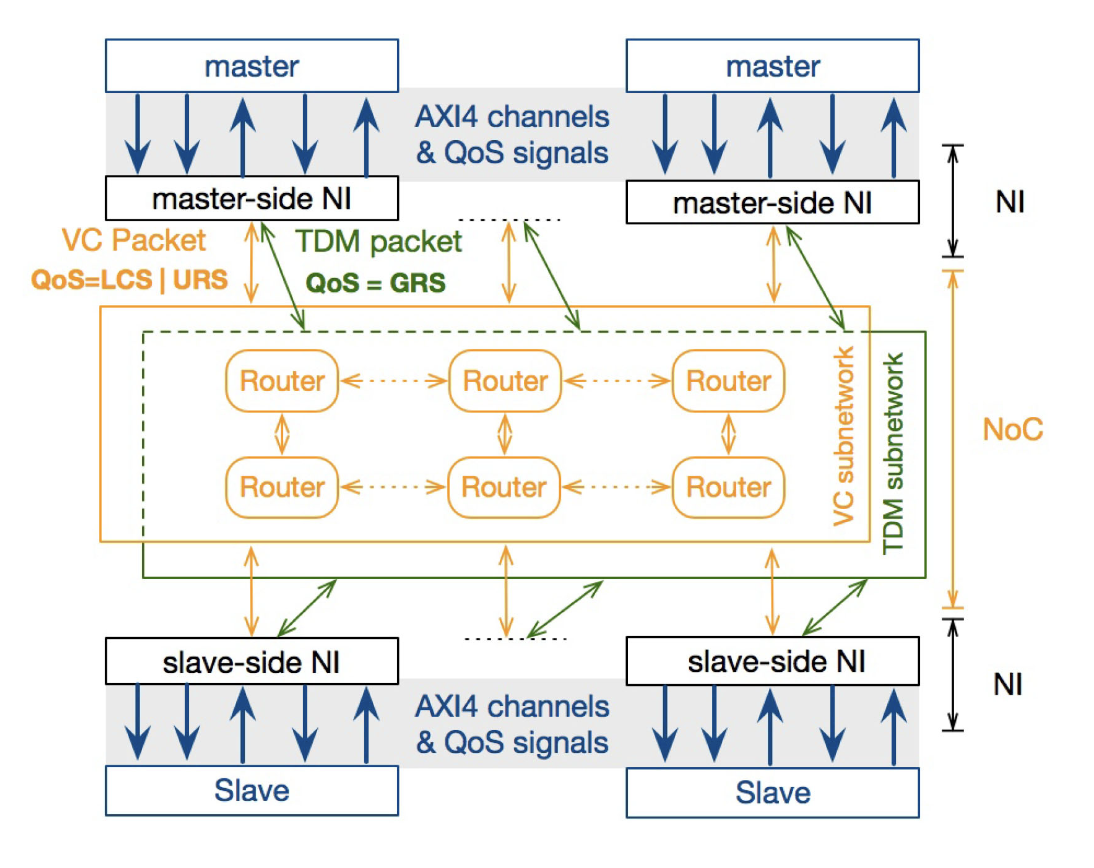
\includegraphics[width=0.95\textwidth]{img/System Architecture.png}
    \caption{System architecture}
    \label{fig:System_Architecture}
\end{figure}

\begin{itemize}
    \item \textbf{Latency-Critical Service (LCS):}\label{LCS} A low-latency forwarding service designed for bursty but non-streaming message transmissions. It provides fast delivery but does not guarantee bandwidth. Typical use cases include CPU-like masters that require short response times.
    \item \textbf{Guaranteed-Rate Service (GRS):}\label{GRS} A streaming service that ensures guaranteed bandwidth for large-volume data flows. It tolerates moderate latency but requires sustained throughput, as in GPU-like masters or other bandwidth-demanding accelerators.
    \item \textbf{Unspecified-Rate Service (URS):}\label{URS} A best-effort service that relies on currently available resources. It provides neither guaranteed bandwidth nor low latency, but aims at fairness among flows. URS is suitable for I/O interfaces such as SATA or USB.
\end{itemize}

To accommodate these QoS requirements, the system architecture is divided into three main components: (i) AXI4-based master/slave nodes, (ii) network interfaces (NIs) that perform protocol message conversion and QoS mapping, and (iii) the NoC fabric itself, which consists of two subnetworks: a VC-based subnetwork for LCS and URS traffic, and a TDM-based subnetwork for GRS traffic. 
This separation enables the NoC to meet diverse application needs without compromising performance or protocol compliance.


\sh{Message Format Conversion}
Two approaches can be used for message format conversion in AXI4-based NoCs. The first is a direct mapping, where each of the five AXI4 channels is converted into a separate packet format. In this case, the NoC must provide five dedicated paths in both subnetworks, one for each AXI4 channel. Although this preserves the semantics of AXI4, it couples the NoC tightly to the protocol, reduces design flexibility, and leads to poor resource utilization due to missing resource sharing. 
The second approach consolidates AXI4 transactions into four unified packet types: \textit{read request}, \textit{read response}, \textit{write request}, and \textit{write response}. These packets share the same NoC resources and are annotated with a QoS identifier (LCS, GRS, or URS), which determines whether they are routed through the VC or TDM subnetwork. This design choice decouples the NoC from the specifics of the AXI4 protocol, improves resource utilization, and enables compatibility with a wide range of interconnect architectures (e.g., buses or NoCs).
For these reasons, the authors adopt the second approach as the foundation of their high-performance and flexible AXI4-based NoC system. Based on this design, the network interface (NI) fulfills three core functionalities:
\begin{enumerate}
    \item \textbf{Dispatching:} The NI receives signals from the AXI4 channels and NoC subnetworks. 
    Transactions are dispatched either to the appropriate AXI4 channel (read/write) or to the correct NoC subnetwork (VC or TDM) according to their QoS identifier (LCS, GRS, URS).
    \item \textbf{Message format conversion:} The NI translates AXI4 transactions into NoC packets and vice versa, thereby decoupling the NoC fabric from protocol-specific details.
    \item \textbf{QoS inheritance:} On the slave side, response packets inherit the QoS class of their corresponding requests. 
    This ensures that QoS policies are consistently maintained across both request and response paths.
\end{enumerate}

Figure~\ref{fig:message_format} illustrates this process. AXI4 transactions from the five original channels (read address, read data, write address, write data, write response) are mapped into four packet types, labeled with QoS information, and forwarded to the appropriate subnetwork. On the return path, the QoS inheritance mechanism guarantees end-to-end service differentiation across the NoC.

\begin{figure}[htbp]
    \centering
    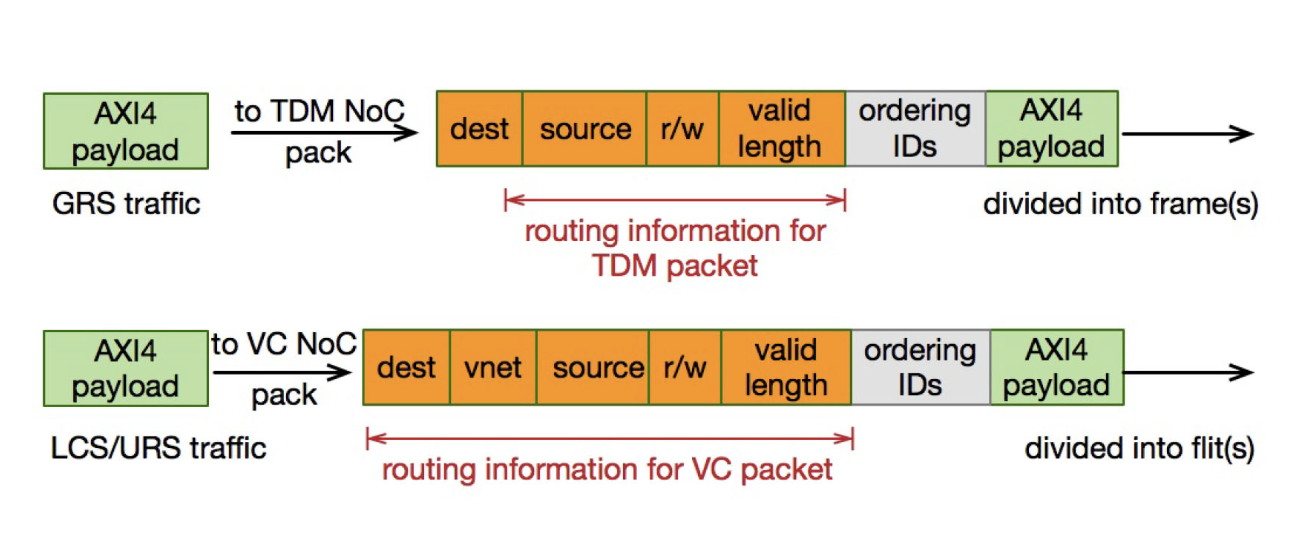
\includegraphics[width=0.95\textwidth]{img/Message format conversion.png}
    \caption{Message format conversion process in the NI}
    \label{fig:message_format}
\end{figure}


\sh{Master-Side and Slave-Side NI Architecture}
The master-side NI (see Figure~\ref{fig:master_NI}) converts AXI4 requests into NoC packets and assigns them to the appropriate subnetwork (VC or TDM) based on their QoS identifier (LCS, GRS, URS). It ensures that transactions are correctly encapsulated and routed to meet the QoS requirements of the originating master (e.g., CPU, GPU, I/O).
The slave-side NI (see Figure~\ref{fig:slave_NI}), on the other hand, unpacks NoC packets into AXI4 responses and delivers them to the slave devices. Since AXI4 response signals do not carry QoS identifiers, the slave-side NI applies a QoS inheritance mechanism, in which the response packet inherits the QoS class of its corresponding request. 
This mechanism guarantees that QoS policies are consistently enforced across both request and response paths, thereby maintaining end-to-end service differentiation in the NoC.

\begin{figure}
    \centering
    \begin{subfigure}[b]{0.48\textwidth}
        \centering
        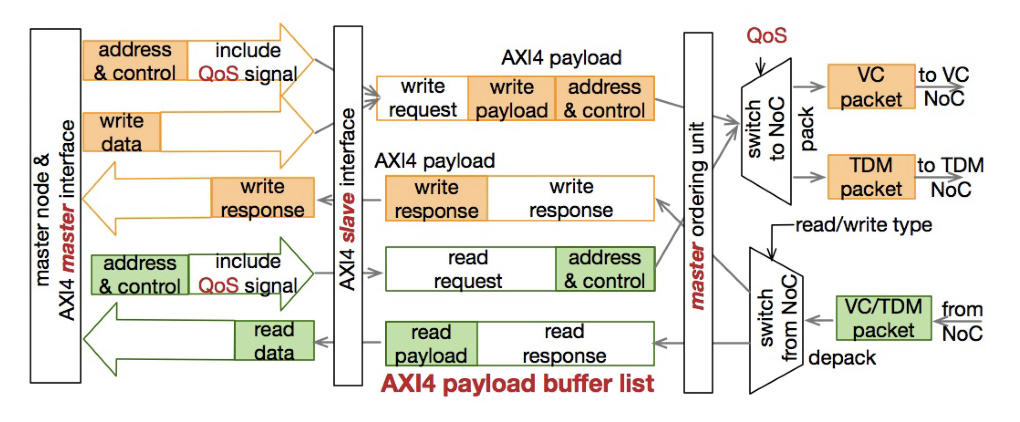
\includegraphics[width=\textwidth]{img/Master-Side_NI.png}
        \caption{Master-Side NI architecture}
        \label{fig:master_NI}
    \end{subfigure}
    \hfill
    \begin{subfigure}[b]{0.48\textwidth}
        \centering
        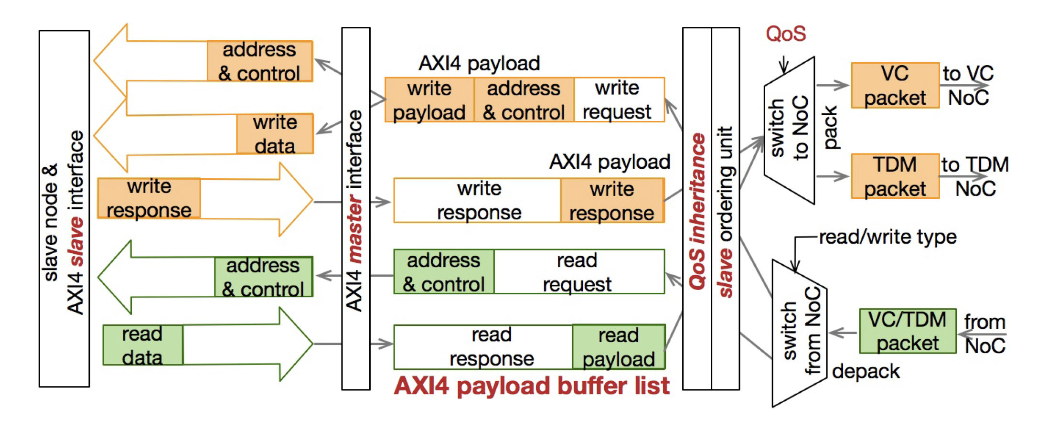
\includegraphics[width=\textwidth]{img/Slave-Side_NI.png}
        \caption{Slave-Side NI architecture}
        \label{fig:slave_NI}
    \end{subfigure}
    \caption{Slave- and Master-Side NI Architectures}
    \label{master_slave_ni}
\end{figure}


\sh{QoS Inheritance}
Because AXI4 response signals do not include QoS identifiers, the NI implements a QoS inheritance mechanism: the response packets automatically inherit the QoS information of their corresponding request packets. This ensures consistent QoS handling across request/response transactions.


\sh{Role of two Subnetworks (VC and TDM)}
To efficiently support heterogeneous QoS requirements, the NoC employs a dual-subnetwork structure:
\begin{itemize}
    \item The \textbf{VC subnetwork} (Virtual Channel) is used for LCS and URS packets. It provides low-latency transmission for critical traffic and fair, best-effort service for background traffic. Several flow control schemes are supported, ranging from strictly separated VCs for different QoS classes to shared VC approaches with priority arbitration.
    \item The \textbf{TDM subnetwork} (Time Division Multiplexing) is dedicated to GRS packets. By pre-allocating both paths and time slots, it guarantees bandwidth and ensures predictable latency for streaming traffic.
\end{itemize}
The separation into VC and TDM subnetworks prevents interference between different QoS services and allows resources to be allocated more effectively.


\sh{Flow Control Mechanisms in VC Subnetwork}  
To manage virtual channel (VC) allocation and arbitration between latency-critical (LCS) and best-effort (URS) packets, four distinct flow control schemes are proposed. The \textit{Individual} scheme assigns dedicated VCs to each virtual network (VN), with LCS packets given higher priority. In the \textit{Individual\_Shared} scheme, all VCs are accessible to LCS packets, while URS packets are confined to a single fixed VC; LCS traffic continues to receive preferential treatment. The \textit{Total\_Shared} scheme allows both LCS and URS packets to share all VCs, although LCS packets are still prioritized during arbitration. Finally, the \textit{Standard} scheme treats all packets equally, with no prioritization across shared VCs. Among these, experimental evaluations indicate that the \textit{Individual\_Shared} scheme delivers the most favorable latency performance for LCS traffic.


\sh{Static Routing in TDM Subnetwork}  
The time-division multiplexing (TDM) subnetwork employs a static routing strategy based on a time-slot-driven routing table, which is constructed using a depth-first search algorithm. This approach enables the precomputation of routing paths, thereby eliminating runtime contention. Each router operates with synchronized time slots to deterministically forward packets, ensuring consistent and predictable delivery. The routing algorithm is designed to support round-trip communication while maintaining guaranteed bandwidth for streaming traffic. As a result, this static routing mechanism effectively minimizes latency and upholds the quality-of-service (QoS) requirements for guaranteed-rate service (GRS) flows.


\sh{Traffic Converter}
A key element of the NI is the \textit{Traffic Converter}, which dynamically balances the load between the two subnetworks: the VC (Virtual Channel) subnetwork and the TDM (Time-Division Multiplexing) subnetwork.
\begin{itemize}
    \item \textbf{VC to TDM Conversion:} When the VC subnetwork experiences congestion, selected latency-critical (LCS) packets are redirected to the TDM subnetwork. These packets are stored in a dedicated FIFO (GRS\_LCS FIFO) and scheduled with lower priority than native guaranteed-rate (GRS) traffic to preserve bandwidth guarantees.
    \item \textbf{TDM to VC Conversion:} If the TDM subnetwork is congested and VC is underutilized, GRS packets may be offloaded to the VC subnetwork. A controller estimates the queuing delay and determines whether rerouting will reduce latency. Converted packets are stored in the LCS\_GRS FIFO and fairly arbitrated with native LCS traffic.
\end{itemize}
This bidirectional conversion mechanism is implemented after the switch-to-NoC unit and before packetization, allowing real-time traffic adaptation. It improves overall utilization, reduces packet latency, and enhances throughput while maintaining QoS guarantees across traffic classes.




\chapter{Results of proposed architecture}

\subsection{Simulator}
The authors developed a custom simulator, shown in Fig.~\ref{fig:simulator_architecture} that supports AXI4, a dual-subnetwork NoC architecture, and three QoS schemes simultaneously. The simulator is built upon the well-known \textit{BookSim2}\TODO{add reference} and \textit{Gem5}\TODO{add reference} frameworks.
The implementation, written in C++, models a system consisting of 168 nodes, two subnetworks, and eight off-chip memory controllers. The design is divided into four identical subareas, each organized as a $7 \times 6$ mesh structure, where every node is connected to a router.
Each node comprises a processor, a private L1 cache, a shared L2 cache, and both a master-side and slave-side network interface (NI). Consequently, every node is capable of functioning simultaneously as a master and a slave. Additionally, each subarea includes two off-chip memory controllers, which are connected to the central routers within the subarea.

\begin{figure}[htbp]
    \centering
    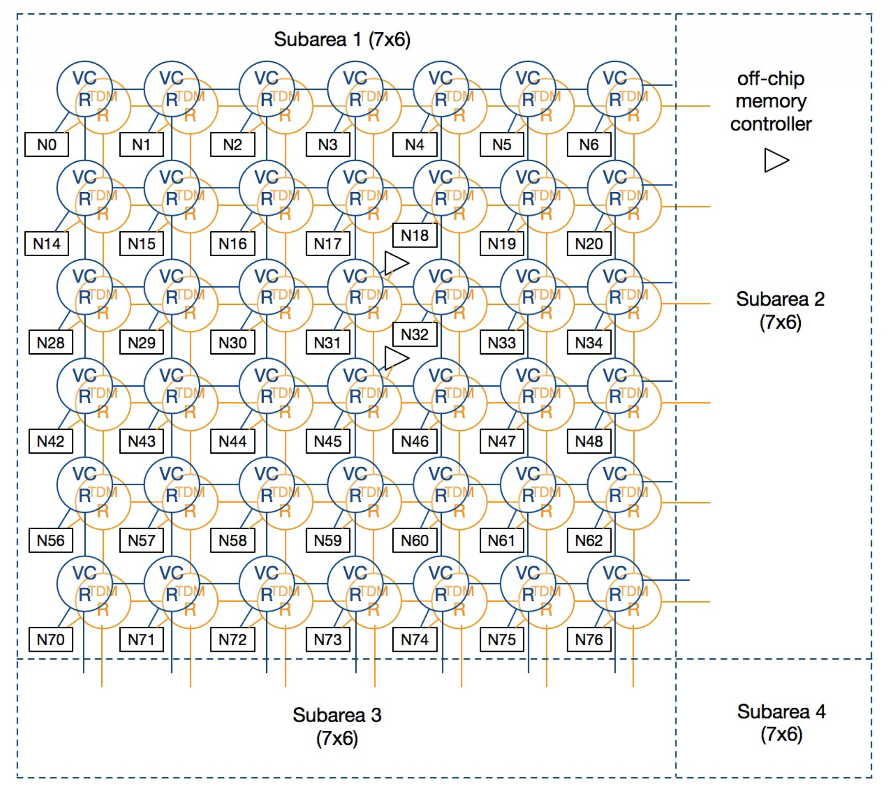
\includegraphics[width=0.95\textwidth]{img/Simulator_Architecture.png.png}
    \caption{Simulator Architecture}~\cite{abderazek_multicore_2013}\label{fig:simulator_architecture}
\end{figure}

The VC network is based on \textit{Gem5}, but for ease of implementation it adopts a cycle-triggered model similar to \textit{BookSim2}, rather than the event-triggered approach used in \textit{Gem5}. The TDM network, by contrast, has a simpler architecture, which facilitates straightforward comparison. 
The network interface (NI) is customized to support the AXI4 protocol. 
Therefore, the results obtained from the proposed simulator can be directly compared with those generated by \textit{Gem5} and \textit{BookSim2}, provided that their NoCs are instantiated with the same configuration.

To regulate the overall injection rate, including LCR, URS, and GRS, the simulator employs a two-level Markov Modulated Process (MMP) model in each traffic generator. The external MMP models the state of a process or thread, whose execution interval varies from nanoseconds to milliseconds. The internal MMP, in turn, models the injection state of request messages during the execution of a process or thread. The parameters $\alpha$ and $\beta$ of the MMP are set according to real-world thread behavior, reflecting both the processing interval and the message injection rate during execution. 

The QoS tag for each request is assigned randomly, based on predefined rates. As a result, a processor is restricted to generating one or two types of QoS schemes, similar to processors in real-world systems. 
The address of each request is also randomly generated from the processor’s communication pairs, which record possible interactions between master and slave nodes. 
Since the influence of the AXI4 ordering requirement is not discussed in this work, the request ID is also selected randomly. This means that ordering constraints may exist for some requests; however, these constraints do not affect the performance of the NoC interconnect, as ordering units are excluded from consideration.

The proposed simulator models a $14 \times 12$ mesh NoC topology, where the average hop count across all requests is four. The TDM period consists of 64 slots (i.e., 64 simulation cycles, one cycle per slot). The VC subnetwork includes two virtual networks, each employing an individual flow control mechanism\TODO{add footnote about alternatives}. 
Each virtual network contains one virtual channel (VC) for LCS packets and one VC for URS packets, with a buffer depth of four flits\TODO{define flit}. The VC router is implemented as a two-stage pipeline, with each stage and each link transfer incurring one cycle of latency. 

The NI can operate at up to 600~MHz in 40-nm technology, but is modeled at 500~MHz in the simulator. To align with the 2~GHz global clock, the NI pipeline latency is scaled from one to four NoC cycles, without impacting subnetwork latency. 
Furthermore, the NI channel width is doubled from 128 to 256 bits, enabling 128~Gb/s throughput, which exceeds the 117~Gb/s maximum throughput requirement of the 2~GHz subnetworks.


\subsection{Experimental Results}





\chapter{Conclusion and critical reflexion}

\sh{Conclusion}
In this paper, a flexible and efficient QoS provisioning scheme was presented for AXI4-based NoC architectures. The proposed design introduces a network interface (NI) capable of AXI4-to-packet conversion, a QoS inheritance mechanism for round-trip support, and a dual-subnetwork structure consisting of a VC-based wormhole network and a TDM-based virtual-circuit network.  

Experimental results demonstrate that the architecture achieves high throughput (up to 19{,}652~Gb/s), low latency for latency-critical flows, and effective traffic balancing through a traffic converter. The system therefore satisfies heterogeneous QoS requirements for CPU-like, GPU-like, and I/O devices within a single unified architecture.

\sh{Critical Reflection}
Although the proposed approach successfully supports three distinct QoS schemes and offers clear performance benefits, several limitations remain:

\begin{itemize}
    \item \textbf{Complexity:} The introduction of dual subnetworks and traffic converters increases hardware and design complexity, potentially impacting scalability and implementation cost.  
    \item \textbf{Simulation scope:} Experiments relied on synthetic traffic generators; while the two-level MMP model is more realistic than conventional models, validation under full application-driven benchmarks (e.g., real workloads) remains necessary.  
    \item \textbf{Dynamic adaptability:} The traffic converter relies on predefined thresholds and rules for switching packets between subnetworks. More advanced, runtime-adaptive methods (e.g., machine learning-based controllers) could further optimize latency and throughput.  
\end{itemize}

These points highlight promising directions for extending the system towards industrial deployment and real-world applications.

\sh{Evaluation}
Overall, the paper makes a strong contribution by bridging the gap between the AXI4 protocol’s QoS requirements and efficient NoC design. Compared to existing works, it uniquely integrates three QoS services, a robust NI design, and an effective load-balancing mechanism. The experimental evaluation shows tangible performance improvements with reasonable hardware overhead. 

However, the work could be strengthened by including comparisons against more application-specific benchmarks, a deeper analysis of area/power trade-offs, and implementation studies in advanced process technologies.  
Despite these limitations, the architecture establishes a flexible framework for next-generation SoCs where heterogeneous cores and devices demand simultaneous support for low latency, guaranteed bandwidth, and best-effort services. It therefore represents a valuable step towards scalable and QoS-aware NoC-based communication infrastructures.


%\input{fundamentals}

%\input{method}

%\input{implementation}

\ifdefined\WITHEVALUATION
%\input{evaluation}
\fi

%\chapter{Conclusion}

\section{Wertung/ Schwachstellen}

\section{Kritische Reflexion}

\cleardoublepage

%\input{glossary}
\clearpage

\listoffigures
\clearpage

\listoftables
\clearpage

\appendix
%\include{appendix_a}
%\include{curriculum_vitae}

%\printbibliography
\MakeBibliography[nosplit]

\end{document}
